%!TEX root = uw-ethesis.tex
% chktex-file 46 (ignore warnings about $...$)
% chktex-file 24 (ignore \label warning)
% chktex-file 35 (ignore max/min)
% chktex-file 44 (ignore warnings about vertical lines in arrays)
\chapter{Quadrotor Motion Planning}\label{chap:quad}



%%%%%%%%%%%%%%%%%%%%%%%%%%%%%%%%%%%%%%%%%%%%%%%%%%%%%%%%%%%%%%%%%%%%%%%%%%%%%%%%
%%%%%%%%%%%%%%%%%%%%%%%%%%%%%%%%%%%%%%%%%%%%%%%%%%%%%%%%%%%%%%%%%%%%%%%%%%%%%%%%
\section{Quadrotor Model}
%%%%%%%%%%%%%%%%%%%%%%%%%%%%%%%%%%%%%%%%%%%%%%%%%%%%%%%%%%%%%%%%%%%%%%%%%%%%%%%%
%%%%%%%%%%%%%%%%%%%%%%%%%%%%%%%%%%%%%%%%%%%%%%%%%%%%%%%%%%%%%%%%%%%%%%%%%%%%%%%%

Quadrotors, as discussed in \autoref{chap:intro}, are growing in popularity for their many uses. Autonomous navigation for quadrotors is still in the early stages of development, although there are already some basic autonomous behaviours in use commercially; for example, many drones now support following a moving person to capture video footage. What makes quadrotor motion planning a truly interesting challenge is the fact that they occupy a 12D state space, and they are non-holonomic vehicles that are governed by nonlinear dynamics. The combination of high-dimensionality and nonlinearity render many current methods ineffective in the context of motion planning, for example the interval method~\cite{jaulin2001,Li2018}, which discretizes the state and control space with intervals, and suffers from the curse of dimensionality~\cite{Indyk1998}.

Before proceeding to the mathematics involved, it may be of interest to the reader to discuss our choice to use the term ``quadrotor''. But first, we begin by seeing that the word ``helicopter'' can be broken down into ``helico'', which is itself a combining form of ``helix'' (screw), and ``pter'' meaning ``wing''. Some people have referred to four-rotor helicopter UAVs as ``quadcopters'', but this terminology is ignorant of the Ancient Greek etymology of such words, as ``heli/copter'' is not the correct partitioning of the English word. So, the term ``quadrotor'' avoids the issue altogether, and its meaning is self-evident.

Now, in order to overcome the hurdles inherent in motion planning for such a complex system as a quadrotor, Ross Allen and Marco Pavone put forth a ``full-stack approach'' for real-time kinodynamic planning of such aerial vehicles~\cite{Allen2016}. First and foremost, a sampling-based planning approach was deemed necessary to deal with unknown environments online, and while \gls{sst}* can handle the high-dimensionality and nonlinearity of the quadrotor system without needing a steering function, the incremental nature cripples its ability to plan effectively in an online setting. On the other hand, \gls{fmt}, with its pre-sampled states and its flexibility in allowing to perform much of the necessary pre-computation offline, is much more suited to online planning. For this reason, the authors centre their planning framework around a variant of FMT* called \texttt{kinoFMT}, introduced in \autoref{chap:prelims}. Once an approximate trajectory is found using this planning algorithm, trajectory smoothing is applied, and due the differentially flat nature of the quadrotor dynamics, it is then feasible to track the smooth trajectory with the proposed controller.

This chapter begins by analyzing the dynamical system that models quadrotor dynamics. Then, much of the work from~\cite{Allen2016} is described in various levels of detail, and conclusions are drawn from the efficacy of this approach. Finally, the main idea of using high-level temporal logic specifications using an abstracted Kripke structure, presented in \autoref{chap:sstpaper}, is applied to quadrotor kinodynamic planning \emph{with} steering under the aforementioned real-time planning framework.





\subsection{Background}

Before delving into the laws of motion for quadrotor systems, we begin by defining the underlying coordinate systems used in our analysis. In order to describe the position and velocity of the quadrotor, we need a fixed inertial reference frame (sometimes called the world frame) where Newton's laws hold. We will use the usual $x,y,z$ coordinates with basis vectors $\{e_1, e_2, e_3 \}$, where ${e_1 = {[1, 0, 0]}^\top}$, ${e_2 = {[0, 1, 0]}^\top}$, and ${e_3 = {[0, 0, 1]}^\top}$. It is worth noting that much of the aviation/aeronautics literature uses the \gls{ned} configuration, so equations of motion found in that frame will differ slightly from those that we will present here. Along with the inertial frame, we define a body-fixed frame with basis $\{b_1, b_2, b_3\}$ whose origin coincides with the centre of mass of the quadrotor. The vectors $b_1$ and $b_2$ lie in the plane formed by the four rotors, and $b_3$ points in the direction opposite the applied thrust. See \autoref{fig:frames}.

\begin{figure}[ht]
    \centering
    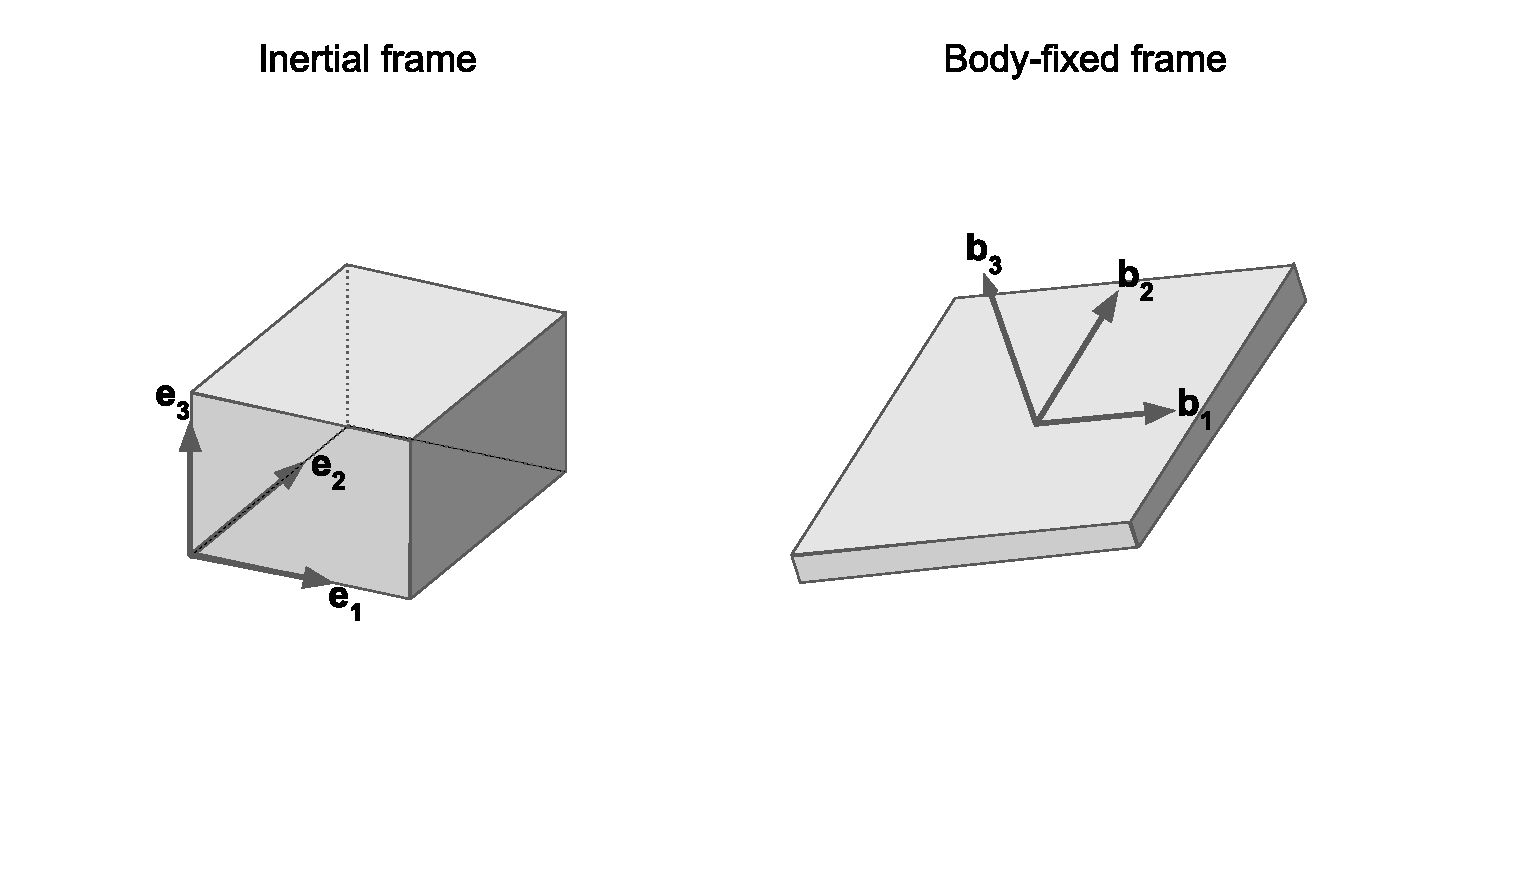
\includegraphics[scale=0.6]{./figures/frames2.eps}
    \caption[Inertial and body-fixed frames]{The inertial frame and the body-fixed frame are shown, where the origin of the body-fixed frame is placed at the centre of mass of the quadrotor, which is represented as a flattened rectangular prism.}
\label{fig:frames}
\end{figure}

Controlling a quadrotor involves adjusting the thrust applied to each of the four rotors. Note that opposite rotors rotate in the same direction, and adjacent rotors rotate in opposite directions; consequently, if all four rotors apply the same amount of thrust, the quadrotor will fly directly upward, and the angular momentum contributed by each rotor cancels so that there is zero rotational motion. Quadrotor motion is described in the space of all rigid body transformations, namely the special Euclidean group $\text{SE}(3)$. This space has six degrees of freedom: translation in three dimensions, and rotation about each of the three body-fixed axes. It bears mentioning that, since there are only four control inputs compared with six degrees of freedom, the quadrotor system is underactuated.

Rotational motion is often described by the Euler angles measuring yaw (about $b_3$), pitch (about $b_2$), and roll (about $b_1$). The use of Euler angles as state variables is not ideal, though, as singularities and jump-discontinuities arise as a result of restricting the domain of such angles. Recent work by Taeyoung Lee et al.\ instead takes a geometric control approach with a globally defined model to avoid many of the issues inherent to Euler angles~\cite{Lee2010}, and we will make use of their work in modeling quadrotor dynamics. The important change they make is to replace the three Euler angle state variables with a single $3 \times 3$ matrix in the special orthogonal group, $\text{SO}(3)$, defined as follows:
\begin{equation}
    \text{SO}(3) = \{ R \in \R^{3 \times 3} \ \vert \ R^\top R = I,\ \det(R) = 1 \}.
\end{equation}
The elements $R \in \text{SO}(3)$ are called rotation matrices, and they are orthogonal matrices that describe the attitude of the quadrotor. Note that the restriction on the determinant of the matrices excludes orthogonal matrices with determinant equal to $-1$, which have the effect of transforming via reflection as opposed to rotation. As we are concerned only with physically possible transformations, reflections are removed from the set of allowed transformation matrices, and the qualifier ``special'' is prepended to the orthogonal group. 

The rotation matrices in $\text{SO}(3)$ are linear transformations that act on vectors via multiplication to produce a rotated vector. Given a vector $\vec{v} \in \R^3$ in the inertial frame (i.e., $v = ae_1 + be_2 + ce_3$ for some $a,b,c \in \R$) and rotation matrix $R \in \text{SO}(3)$, $w=Rv$ is the result of rotating $v$ by $R$, where $w$ is expressed in the inertial frame. A useful interpretation of such rotation matrices is that the matrix $R$ represents the current orientation of a rigid body. That is to say, the body-fixed axes are obtained, as above, by applying the rotation $R$ to each of the basis vectors $e_1, e_2$, and $e_3$. In this way, we need not consider the rotation an active change in the quadrotor's orientation, but rather as the current orientation obtained by rotating the axes of the inertial frame.





\subsection{Dynamics}\label{quad:dynamics}

We are now sufficiently equipped to outline the equations of motion of a quadrotor \gls{uav}. The first equation states the relationship between the position of the centre of mass, ${x={[x_1, x_2, x_3]}^\top \in \R^3}$, and the velocity of the centre of mass, $v={[v_1, v_2, v_3]}^\top \in \R^3$, together constituting the first six state variables. The equation is simply
\begin{equation}
    \dot x = v.\label{quad:dyn:eqn1}
\end{equation}

To develop the next, more interesting, equation, we begin by noticing that $b_3 = Re_3$. If we express the magnitude of the thrust generated by the $i^{th}$ propeller as $f_i,\ i \in \{1,2,3,4\}$, then the total thrust in the body-fixed frame is given by $fb_3$, where $f = \sum_{i=1}^4 f_i$. Therefore, in the inertial frame, the total thrust is written as $fRe_3$. The only other force acting on the quadrotor (ignoring disturbances) is the force of gravity, which pulls along the $-e_3$ axis, and we write the force as $-mge_3$, where $m$ is the mass of the quadrotor, and $g$ is the magnitude of the force of gravity ($g \approx 9.8$ on the surface of the Earth). Using Newton's Second Law, we may now put these forces together to write our second equation of motion,
\begin{equation}
    m\dot v = fRe_3 - mge_3.\label{quad:dyn:eqn2}
\end{equation}

The final two equations of motion for the quadrotor system describe the rotational dynamics. Define $\Omega \in \R^3$ to be the angular velocity of the quadrotor in the body-fixed frame. $R$ and $\Omega$ constitute the remaining state variables, and they appear together in an interesting way in the third equation of motion, which describes the rate at which the rotation matrix changes with time.

Before proceeding, let us first introduce $\mathfrak{so}(3)$, the Lie algebra associated with the Lie group $\text{SO}(3)$. A Lie algebra contains the elements of the tangent space of the Lie group at the identity, and in this case, we have that $\mathfrak{so}(3)$ is simply the set of skew-symmetric matrices,
\begin{equation}
    \mathfrak{so}(3) = \{ X \in \R^{3 \times 3} \ \vert \ X^\top + X = 0 \}.
\end{equation} 
The skew-symmetric matrices represent infinitesimal rotations. Consider rotating a vector $x$ about some unit vector, $v$, by angle $\theta$ in the counterclockwise direction. In the limit as $\theta$ approaches $0$, the rotation occurs normal to the plane containing both vectors, in the direction $v \times x$. This motivates the definition of the \emph{hat map}, $\hat \cdot : \R^3 \to \mathfrak{so}(3)$ which satisfies $\hat a b = a \times b$\ for all $a, b \in \R^3$.
\begin{equation}
    \hat a
    =
    \widehat{
    \begin{bmatrix}
        a_1 \\
        a_2 \\
        a_3
    \end{bmatrix}
    }
    =
    \begin{bmatrix}
        0        &  -a_3 & a_2 \\
        a_3 &  0         & -a_1 \\
        -a_2 & a_1  & 0
    \end{bmatrix}
\end{equation}
Tying these concepts together, the infinitesimal generator of rotation in the given scenario is the matrix $\hat v$, since $\hat v x$ yields the direction of the rotation of $x$ about $v$ by an infinitesimal angle.

Recall that an element $\hat v \in \mathfrak{so}(3)$ is in the tangent space of $\text{SO}(3)$ \emph{at the identity}. In order to produce an infinitesimal rotation at an arbitrary element $R \in \text{SO}(3)$, we simply left-multiply the appropriate infinitesimal rotation (element of $\so(3)$) by $R$. In this case, $\hat \Omega$ is the appropriate element of $\mathfrak{so}(3)$ since $\Omega$ describes the rotational motion, and thus the axis of rotation, of the quadrotor. Therefore, we conclude that the third equation of motion is:
\begin{equation}
    \dot R = R \hat \Omega.\label{quad:dyn:eqn3}
\end{equation}

Finally, the last equation of motion governs how $\Omega$ changes over time. Given the moment of inertia matrix, $J \in \R^{3 \times 3}$, of our quadrotor, we can write an equation for the total torque in the body-fixed frame, $\tau \in \R^{3 \times 3}$ (the rotational analog to the second equation of motion, \autoref{quad:dyn:eqn2}). Following the same line of reasoning in deriving \autoref{quad:dyn:eqn3}, we can see that the rate of change of any one body-fixed frame basis vector, $u \in \{b_1, b_2, b_3\}$, due to the angular velocity is given by
\begin{equation}
    \frac{du}{dt} = \Omega \times u = \hat \Omega u.\label{quad:eqn:dudt}
\end{equation}
For any differentiable vector-valued function $f(t) = f_x(t)b_1 + f_y(t)b_2 + f_z(t)b_3$, we can use \autoref{quad:eqn:dudt} to find the time-derivative of $f$ as follows~\cite{Lanczos1986}:
\begin{align*}
    \frac{df}{dt} &= \frac{df_x}{dt}b_1 + f_x\frac{db_1}{dt}
                    +\frac{df_y}{dt}b_2 + f_y\frac{db_2}{dt}
                    +\frac{df_z}{dt}b_3 + f_z\frac{db_3}{dt} \\
                  &= \frac{df_x}{dt}b_1 + \frac{df_y}{dt}b_2 + \frac{df_z}{dt}b_3
                    +\Omega \times (f_x(t) b_1 + f_y(t) b_2 + f_z(t) b_3) \\
                  &= {\left( \frac{df}{dt} \right)}_b + \Omega \times f(t),
\end{align*}
where ${\left( \frac{df}{dt} \right)}_b$ indicates the derivative of $f$ as seen in the body-fixed frame. Note that an observer in the body-fixed frame does not perceive
The last remaining concept that needs to be defined to obtain the remaining equation of motion is the angular momentum, $L$, which satisfies $L = J\Omega$. The time-derivative of angular momentum is equal to the total torque, $\tau = {[\tau_1, \tau_2, \tau_3]}^\top$ (in the body-fixed frame), which is exactly what we use to determine an equation for $\dot \Omega$.
\begin{align*}
\tau &= \frac{dL}{dt} \\
     &= \frac{d}{dt} J\Omega \\
     &= {\left( \frac{d}{dt} J\Omega \right)}_b + \Omega \times J\Omega \\
     &= J\dot\Omega + \Omega \times J\Omega
\end{align*}
Note that in the last step, since the derivative is taken in the body-fixed frame, the moment of inertia, $J$, does not change, so the term $\dot J\Omega$ resulting from the product rule vanishes. Rearranging, we obtain our final equation of motion:
\begin{equation}
 J\dot \Omega = \tau - \Omega \times J\Omega. \label{quad:dyn:eqn4}
\end{equation}

We summarize the nonlinear dynamics of the deterministic model for quadrotor motion below~\cite{Mellinger2012}.
\begin{equation}
    \begin{aligned}
        \dot x &= v \\
        \dot v &= \frac{f}{m}Re_3 - ge_3 \\
        \dot R &= R \hat \Omega \\
        \dot \Omega &= J^{-1} (\tau - \Omega \times J\Omega)
    \end{aligned}
\label{quad:full_dyn}
\end{equation}

The inputs to this system are $u={[f, \tau_1, \tau_2, \tau_3]}^\top \in \R^m$ with dimension $m=4$, and the state vector is given by $X = {[x, v, R, \Omega]}^\top \in \R^3 \times \R^3 \times \text{SO}(3) \times \R^3$.

Note that the low-level quadrotor controller must convert the input values to the individual torques to be applied to each propeller. We assume that the first and third propellers rotate clockwise, the second and fourth propellers rotate counterclockwise, and that the torque is directly proportional to the thrust generated by a propeller, with proportionality constant $c_\tau$. Recall that $f_i, \ i \in \{1,2,3,4\}$ denote the thrusts generated, and define $d$ to be the distance in the $b_1b_2$-plane from the centre of mass to the centre of each propeller. Then, we can write the inputs as follows~\cite{Lee2010, Mellinger2012}:
\begin{equation}
    \begin{bmatrix}
        f \\ \tau_1 \\ \tau_2 \\ \tau_3
    \end{bmatrix}
    =
    \begin{bmatrix}
        1       & 1       & 1       & 1   \\
        0       & -d      & 0       & d   \\
        d       & 0       & -d      & 0   \\
        -c_\tau & c_\tau  & -c_\tau & c_\tau
    \end{bmatrix}
    \begin{bmatrix}
        f_1 \\ f_2 \\ f_3 \\ f_4
    \end{bmatrix}.
\label{quad:eqn:invert_this}
\end{equation}
Since this matrix is invertible provided $d, c_\tau \neq 0$, it suffices to invert the matrix and multiply by the vector of inputs, $u$, in order to obtain the necessary thrusts, and therefore torques, for the individual propellers.

The remainder of this chapter solves the following problem, as similarly stated in~\cite{Allen2016}, with the addition of satisfying a temporal logic specification.
\begin{problem}
    \  \\
    Let $\mathcal{X}_{free} \subseteq \R^3 \times \R^3 \times \text{SO}(3) \times \R^3$ be the subset of state space that is unobstructed, and let $\mathcal{U} \subseteq \R^4$ be the set of admissible control inputs. Furthermore, let $\Phi$ be a deterministic \mucalc{} specification. Then, given the continuous-time quadrotor dynamical system,
    \begin{equation}
        \dot X(t) = f(X(t), u(t)),\hspace{4mm} X(0) = X_0,\label{quad:generic_sys}
    \end{equation}
    where $f$ is given by the equations of motion in \autoref{quad:full_dyn},
    determine a control signal,
    \begin{equation}
        u(t) = {[f(t), \tau_1(t), \tau_2(t), \tau_3(t)]}^\top \in \mathcal{U},
    \end{equation}
    and corresponding state trajectory, 
    \begin{equation}
        X(t) = {[x(t), v(t), R(t), \Omega(t)]}^\top \in \mathcal{X}_{free}
    \end{equation}
    that satisfies specification $\Phi$, or return failure if such a trajectory is not found.
\label{quad:problem}
\end{problem}




%%%%%%%%%%%%%%%%%%%%%%%%%%%%%%%%%%%%%%%%%%%%%%%%%%%%%%%%%%%%%%%%%%%%%%%%%%%%%%%%
%%%%%%%%%%%%%%%%%%%%%%%%%%%%%%%%%%%%%%%%%%%%%%%%%%%%%%%%%%%%%%%%%%%%%%%%%%%%%%%%
\section{Real-Time Motion Planning}\label{chap:quad:rtmp}
%%%%%%%%%%%%%%%%%%%%%%%%%%%%%%%%%%%%%%%%%%%%%%%%%%%%%%%%%%%%%%%%%%%%%%%%%%%%%%%%
%%%%%%%%%%%%%%%%%%%%%%%%%%%%%%%%%%%%%%%%%%%%%%%%%%%%%%%%%%%%%%%%%%%%%%%%%%%%%%%%

As discussed in \autoref{chap:prelims} and \autoref{chap:sstpaper}, many motion planning algorithms require knowledge of a steering function. \texttt{kinoFMT} (\autoref{alg:fmt}) is one such algorithm, but as previously noted, the nonlinear quadrotor dynamics make it difficult (or perhaps impossible) to find an analytic solution to the \gls{obvp}. In order to apply the \texttt{kinoFMT} algorithm to the problem of kinodynamic planning for a quadrotor, we must therefore use an approximation to the 12D nonlinear system that has a known steering function. The crucial property involved in using an approximation to the full dynamics is called \emph{differential flatness}, which allows any sufficiently smooth path to be tracked. The method employed by Allen et al.~\cite{Allen2016} involves two further important steps: reachable set approximation, and trajectory smoothing. To elaborate, the reachable set approximation is arguably the key step that allows for online planning, as it is used to rapidly connect the initial state and goal states to the preexisting tree that is to be computed beforehand offline. Once a path is planned between the newly added initial state and goal states, a smooth path is generated called a \emph{minimum-snap trajectory}, and we leverage the differential flatness property of the quadrotor dynamics to be able to track this smooth path in the full dynamics. The details involved in tracking are provided, and simulations are performed to demonstrate the effectiveness of this method.





\subsection{Framework Overview}

We now outline the high-level real-time planning framework proposed in~\cite{Allen2016}. The entire process is broken down into two parts: the offline precomputation phase, where as much information as possible is gathered before knowing any of the specific details that will become clear during real-time trials, and the online planning phase, which takes into account the actual initial position and goal region and performs the various planning steps described in later sections.



\subsubsection{Offline Phase}

Before online planning can begin, it is desirable to perform as much precomputation as possible to minimize the computational effort, and therefore the time, required when online. With this in mind, there are three steps to perform offline:
\begin{enumerate}
    \item sampling the state-space,
    \item constructing a cost roadmap,
    \item training a classifier that determines nearest nodes.
\end{enumerate}

The sampling step simply stores a user-defined number of samples, $N$, in a set, $V$. The samples are drawn uniformly from the unobstructed state-space, without any regard for potential obstacles (as such information is as yet unknown). This manner of sampling is a boon to the flexibility of the proposed method, as it can be applied online in a very general setting.

Next, for every pair of states in $V$, the \gls{obvp} is solved. The optimal time and cost are then stored as values in a look-up table (or dictionary), called \texttt{Cost}, associated with the corresponding pair of states. In this way, no computation for cost is required while running \texttt{kinoFMT} online, except when it comes to pairs involving the states known only when online: the initial state and sampled goal states. This issue is addressed in the final step of the offline phase.

Note that as $N$ gets large, the number of pairs grows quadratically as $N(N-1)$, and the bisection optimization method used to compute the optimal time for each pair converges linearly. For $N>2000$, this can be rather expensive, so one could choose to instead sample some number of pairs on which to perform the precomputation. Furthermore, the ordering of the pairs matters, so one cannot use a symmetry argument to halve the number of computations. To illustrate this point, consider two states in one dimension (with 2D state-space: position and velocity), each with some positive velocity. The state that is behind has a fairly straightforward means of reaching the other state, whereas the state that is ahead would be forced to change direction, get to the appropriate position and accelerate in the positive direction once again to reach the desired positive velocity.

In order to avoid having to compute the cost between each of the initial or goal states and the existing $N$ samples, which would involve solving the \gls{obvp} $O(N)$ times, a machine learning approach is implemented. A \gls{svm} is used, learning from the data in the \texttt{Cost} look-up table to rapidly classify a pair of points as ``near'' or ``not near'' in terms of the cost incurred by traveling from one state to the other. As such, the \gls{obvp} must be solved only for those points that are estimated to fall within a certain cost threshold.



\subsubsection{Online Planning}

Upon beginning a trial with a quadrotor, the first step is to sample $N_{goal}$ states from the now-known goal region. Then, given the initial state of the quadrotor, we determine the outgoing nearest neighbours from the initial state using the trained \gls{svm} and store them in $\mathcal{N}_{init}^{out}$, and we similarly determine the incoming neighbours for each of the goal states, storing them in $\mathcal{N}_{goal}^{in}$. At this point, the \gls{obvp} is solved between the initial state (goal states) and the states in its neighbourhood, $\mathcal{N}_{init}^{out}$ ($\mathcal{N}_{goal}^{in}$), and the appropriate entries are added to the cost roadmap, \texttt{Cost}. Note that using the \gls{svm} to estimate cost-limited reachable sets provides an immense reduction in the number of online \gls{obvp} solutions required, from $O(N)$ down to $O(1)$.

Now that the \texttt{Cost} look-up table is complete, the \texttt{kinoFMT} algorithm (\autoref{alg:fmt}) is run on the set of samples, $V$ along with the initial and goal states. The algorithm quickly returns the optimal path from start to goal, excluding any paths that are found to collide with obstacles. However, given that the path is found using an approximated linear model, it must be smoothed so that it may be tracked by leveraging the differential flatness of the quadrotor system. With this aim, a smoothing algorithm takes the waypoints (states) from the path outputted by \texttt{kinoFMT} and produces a set of four high-degree polynomials in the flat output variables that are smooth up to fourth order. Finally, all that remains is to track the smooth path using an appropriately tuned feedback controller.
 



\subsection{Differential Flatness}\label{quad:diff_flat}

We say of a system that it is differentially flat if the states and the inputs can be written as functions of the system's flat outputs and their derivatives. We state the definition more precisely as follows~\cite{Greeff2018}:
\begin{defn}
    Consider a continuous-time nonlinear system $\dot x(t) = f(x(t),u(t)),\ x(0) = x_0$ where $t \in \R$, $x(t) \in \R^n$ is the state, $u(t) \in \R^m$ is the input, and $f$ is a smooth function. This nonlinear system is \emph{differentially flat} if there exists $\zeta(t) \in \R^m$, whose components are differentially independent, such that the following hold~\cite{Fliess1995}:
    \begin{align*}
        \zeta &= \Lambda(x, u, \dot u, \mathellipsis, u^{(\delta)}) \\
            x &= \Phi(\zeta, \dot \zeta, \mathellipsis, \zeta^{(\rho-1)}) \\
            u &= \Psi^{-1}(\zeta, \dot \zeta, \mathellipsis, \zeta^{(\rho)})
    \end{align*}
    where $\Lambda, \Phi, \Psi^{-1}$ are smooth functions, $\zeta = {[\zeta_1, \mathellipsis, \zeta_m]}^\top$ is the vector of \emph{flat outputs}, and $\delta$ and $\rho$ are the maximum orders of the derivatives of $\zeta$ and $u$ necessary in defining the flat outputs and their relation to $x$ and $u$.
\end{defn}
The concept of differential flatness is useful for many reasons, although two in particular seem eminently popular in the field of motion planning. The first is that differential flatness can be used in the process of feedforward (or feedback) linearization to separate a nonlinear system into a linear flat model and a nonlinear transformation, so that is possible to consider the control problem only on the linear part, and the resulting flat states and flat inputs can be used to correct for the nonlinear part via inversion of the nonlinear transformation~\cite{Greeff2018,VanNieuwstadt1998}. The second consequence of differential flatness, and the one we focus on here, is that any smooth trajectory in the flat output space, subject to reasonably bounded derivatives, can be tracked~\cite{Mellinger2011}. The significance of this fact is not to be understated, as even the underactuated quadrotor can track a sufficiently smooth path generated from the flat outputs of the system.

In the case of quadrotors, the flat outputs can be chosen to be the position of the centre of mass in the inertial frame and the yaw angle, $\zeta = {[x_1, x_2, x_3, \psi]}^\top$. Mellinger and Kumar prove that this choice of flat outputs does indeed admit a way to write the state and input as a function of $\zeta$ and its derivatives up to fourth order.



\subsection{Quadrotor Dynamics Approximation}

There exist many known approaches to handling nonlinear dynamics when solving motion planning problems, such as using a planner that avoids the steering problem altogether (e.g., \gls{sst}). Another approach, when dealing with a differentially flat nonlinear system, is to use feedforward linearization, as mentioned in \autoref{quad:diff_flat}. In the method presented here, as in~\cite{Allen2016}, the quadrotor system is first approximated to be the linear double integrator system (\autoref{quad:approxdyn}). The approximation assumes the quadrotor can accelerate in any direction at any time, which, while crude, is sufficient to generate high-quality trajectories from an initial state to a goal region. The idea is that, upon using \texttt{kinoFMT} to generate an ordered set of waypoints on this simplified system, a smooth trajectory in the flat outputs can be generated and tracked in the full dynamics.
\begin{equation}
    \dot{\tilde{x}}(t) = 
    \underbrace{
    \begin{bmatrix}
        0_{3 \times 3} & I_{3 \times 3} \\
        0_{3 \times 3} & 0_{3 \times 3}
    \end{bmatrix}
    }_A \tilde{x}(t)
    +
    \underbrace{
    \begin{bmatrix}
            0_{3 \times 3} \\
            I_{3 \times 3}
    \end{bmatrix}
    }_B  \tilde{u}(t)
    -
    \underbrace{
    \begin{bmatrix}
        0_{5 \times 1} \\
        g
    \end{bmatrix}
    }_c
\label{quad:approxdyn}
\end{equation}
Here, $\tilde{x} = {[x_1, x_2, x_3, \dot{x}_1, \dot{x}_2, \dot{x}_3]}^\top \in \R^6$ is simply a truncated representation of the full state including only position and velocity, and $\tilde{u} = {[\ddot{x}_1, \ddot{x}_2, \ddot{x}_3]}^\top \in \R^3$  is the new control. We denote the matrix multiplying $\tilde{x}(t)$ by $A$, the matrix multiplying $\tilde{u}(t)$ by $B$, and the constant vector by $c$.

Now that we are working with a linear system, we solve the \gls{obvp} as in~\cite{Schmerling2015}. Given any two (sampled) states, we seek an analytic solution to the problem of finding an optimal path between them, as well as the optimal control signal used to generate such a path. We begin by defining the cost function
\begin{equation}
    \mathcal{J}(\tilde{u}, t_{f}) = \int_0^{t_f} 1 + {\tilde{u}(t)}^\top R_u \tilde{u}(t) dt
\label{quad:eqn:cost}
\end{equation}
where $R_u \in \R^{3 \times 3}$ is symmetric positive definite, and $t_f$ is the fixed final time. This cost function prioritizes minimum-time solutions while also penalizing control effort. A suitable choice for the control penalty weighting matrix is $R_u = w_R I_{3 \times 3}$, for some $w_R \in \R$.

Without derivation, the optimal cost for the double integrator \gls{obvp} from initial state $\tilde{x}_0$ at time $t=0$ to $\tilde{x}_1$ at time $t=t_f$ is given by~\cite{Schmerling2015, Allen2016}
\begin{equation}
    \mathcal{J}^*(t_f) =
    t_f + {(\tilde{x}_1 - \underbar{x}(t_f))}^\top {G(t_f)}^{-1} (\tilde{x}_1 - \underbar{x}(t_f)).
\label{quad:eqn:opt_cost}
\end{equation}
The state and control trajectories which achieve this optimal cost are given by
\begin{align}
    \tilde{x}(t) &= \underbar{x}(t) + G(t)\exp(A^\top[t_f - t]){G(t_f)}^{-1} (\tilde{x}_1 - \underbar{x}(t_f)) \\
    \tilde{u}(t) &= R_u^{-1} B^\top \exp(A^\top[t_f - t]){G(t_f)}^{-1} (\tilde{x}_1 - \underbar{x}(t_f))
\end{align}
where
\begin{align}
    \underbar{x}(t) &= \exp(At)x_0 + \int_0^t \exp(As)c\ ds \\
               &= \exp(At)x_0
                  -
                  \begin{bmatrix}
                      0 \\
                      0 \\
                      gt^2/2 \\
                      0 \\
                      0 \\
                      gt
                  \end{bmatrix} \\
    G(t)  &= \int_0^t \exp(As)B R_u^{-1} B^\top \exp(A^\top s)\ ds  \\
          &= \frac{1}{w_R}
          \begin{bmatrix}
            t^3/3   &  0  &  0  & t^2/2 &  0  &  0 \\
            0  &  t^3/3   &  0  &  0  & t^2/2 &  0 \\
            0  &  0  & t^3/3   &  0  &  0  & t^2/2 \\
            t^2/2 &  0  &  0  & t  &  0  &  0 \\
            0  & t^2/2 &  0  &  0  & t  &  0 \\
            0  &  0 & t^2/2 &  0  &  0  & t \\
          \end{bmatrix}.
\end{align}

The only remaining unknown is the final time $t_f = \argmin_{t > 0} \mathcal{J}^*(t)$, which can be found via the bisection method performed on the derivative of the convex function $\mathcal{J}^*$. This involves choosing an initial interval $[a,b]$ in which to check for an optimal solution (e.g., $[0.0001, 100]$) as well as some error tolerance, $\epsilon$. The bisection method is a recursive algorithm that checks to see whether the derivative of the function at $a$ has the same sign as the derivative of the function at the midpoint of the interval, $q$. If it is not the same, recurse on the interval $[a,q]$ since a turning point (i.e., a minimum) exists therein. Similarly, if the derivative at $q$ has a different sign from the derivative at $b$, recurse on $[q,b]$. The algorithm terminates and returns the midpoint once the length of the interval, $b-a$, is less than $\epsilon$, or when the derivative at the midpoint is zero.




\subsection{Reachable Set Approximation}\label{quad:reachable_set}


The problem of finding a state $\tilde{x}_b$ that is nearest to state $\tilde{x}_a$ in a kinodynamic framework is not as simple as finding the state $\tilde{x}_b$ which minimizes the Euclidean distance between $\tilde{x}_a$ and $\tilde{x}_b$. Due to the issue of drift, including the consideration of momentum and angular momentum, distance is insufficient in determining the actual difficulty involved in transiting from one state to another. Instead, the cost is given by \autoref{quad:eqn:cost}, used as the optimality condition for the \gls{obvp}. In the same vein, while geometric planners may use some maximal, distance-based search radius, our kinodynamic planner instead uses a cost-limited reachable set when looking for nearby states. We define such a reachable set from a state $\tilde{x}_a$ with maximum cost $J_{th}$, in the subset of unobstructed state space of the approximate dynamics, $\mathcal{\tilde{X}}_{free}$, and given the set of admissible input signals, $\mathcal{\tilde{U}}$, as follows~\cite{Allen2014}:
\begin{equation}
    R(\tilde{x}_a, \mathcal{\tilde{U}}, J_{th}) = 
        \{ \tilde{x}_b \in \mathcal{\tilde{X}}_{free} \ \vert \ \exists \tilde{u} \in \mathcal{\tilde{U}}, t \in [0, t_f]\ \text{s.t.}\ \tilde{x}(t) = \tilde{x}_b\ \text{and}\ \mathcal{J}(\tilde{u},t) \leq J_{th} \}.
\end{equation}
In words, the cost-limited reachable set contains all unobstructed states that can be reached before the final time, $t_f$, using admissible controls and without exceeding the cost threshold.

The issue posed by real-time planning is that solving the \gls{obvp} from the previously unknown initial state to each of the $N$ sampled states is computationally expensive. This would then have to be repeated for each of the newly sampled goal states, rendering the task of online kinodynamic planning practically infeasible. Even worse, if the number of samples is large and the look-up table \texttt{Cost} does not include the cost between every pair of the $N$ samples, then querying for nearby states requires even more \gls{obvp} solutions. What has been proposed in~\cite{Allen2016} is to use an \gls{svm} classifier to estimate whether any given state lies within the cost threshold, $J_{th}$, of another state. That is, when calling $\texttt{Near\_Forward}(x,V,J_{th})$ from \autoref{alg:fmt}, the \gls{svm} is used to estimate, for each $v \in V$, whether or not $v \in R(x, \mathcal{\tilde{U}}, J_{th})$. Similarly, $\texttt{Near\_Backward}(x,V,J_{th})$ returns the set of states $v$ such that $x \in R(v, \mathcal{\tilde{U}}, J_{th})$.

An \gls{svm} works by consuming a large array of training data, \texttt{arr\_train}, with $n_{train}$ entries called \emph{feature vectors}, as well as an array of $n_{train}$ labels. The idea is to train the supervised learning algorithm on the correct labels to be able to partition the space of feature vectors in such a way as to be able to accurately classify new feature vectors. This partitioning can be accomplished in many ways, such as using a simple linear hyperplane as a boundary, or creating more complex nonlinear boundaries. The boundary that is used is determined by the chosen \emph{kernel} function.

Our implementation uses the scikit-learn package ``svm'' for Python. We begin by determining what should be included in the feature vector. One simple choice for the feature vector that is sufficient for our purposes is to concatenate the pair of states. Given a pair of states $(\tilde{x}_a, \tilde{x}_b)$, $\tilde{x}_a, \tilde{x}_b \in \mathcal{\tilde{X}}_{free} \subseteq \R^6$ (in the approximate dynamics), let the $i^{th}$ feature vector of \texttt{arr\_train} be $p_i = {[\tilde{x}_a^\top, \tilde{x}_b^\top]}^\top$. The corresponding label $y_i$ is equal to 1 if the actual optimal cost from $\tilde{x}_a$ to $\tilde{x}_b$ is less than $J_{th}$, and 0 otherwise. In our work, we found the most success using a polynomial kernel of degree 3. All that remains is to choose an error penalty parameter, $C$, as input to the SVC function from the scikit-learn svm package. As with many machine learning techniques, this step is subject to trial and error. Once chosen, the SVC function can be used to train a classifier. Given a new pair of vectors, one can then construct the appropriate feature vector and run it through the trained classifier to check whether or not the pair satisfies the cost-limited reachability condition.

We encourage interested readers to refer to~\cite{Smola2004} for further details regarding \gls{svm}s. 




\subsection{Trajectory Smoothing}

The path generated by \texttt{kinoFMT} cannot be used directly as it is based on the double integrator dynamics approximation\footnote{Note that if we were to apply a different method that could plan on the full nonlinear dynamics, such as with \gls{sst} (\autoref{chap:sstpaper}), smoothing would not be a necessary step, although it can be useful in improving trajectory quality.}. To use the generated path, we must first create a smooth trajectory in each of the four flat outputs: the three components of position and the yaw angle. We opt to use polynomial interpolation on the waypoints of the path generated by our planning algorithm. This section is primarily based on the work of Richter et al.~\cite{Richter2016}, though many details that are missing from these papers are provided.

To accomplish the task of smoothing, we will use $M$ polynomials of order $N_p$ for each of the four flat output variables. To introduce the topic, we will begin by analyzing how the interpolation task is accomplished for one polynomial segment between two waypoints for a single flat output variable. We will then extend the result to create $M$ polynomials, and the procedure may be repeated for each of the other flat output variables.

Based on the proof that the quadrotor system is differentially flat~\cite{Mellinger2011}, it is shown that four derivatives of the flat outputs are required to express the state and the input. For this reason, we require that each polynomial we construct is continuous up to the fourth derivative. Furthermore, each polynomial must have equal derivatives at shared intermediate waypoints to ensure smoothness of the full trajectory. Despite these restrictions, there remain infinitely many possible polynomials that join successive waypoints. We choose the ``best'' option which we define to be the unique polynomial that minimizes the integral of the square of the snap (fourth derivative) of the polynomial, as shown in \autoref{quad:eqn:Jsnap}.
\begin{equation}
    J_{snap}(T) = \int_0^T P^{(4)}(t)dt = p^\top Q(T) p
\label{quad:eqn:Jsnap}
\end{equation}
Here, $T$ is the fixed final time for the given polynomial segment, which was found when solving the \gls{obvp} and subsequently recording the optimal duration and cost in the \texttt{Cost} roadmap, and $Q$ is the Hessian matrix for the integral expression with respect to the vector of polynomial coefficients, $p$. $P(t)$ is given by
\begin{equation}
    P(t) = \sum_{i=0}^{N_p} p_i t^i \hspace{2mm},
    \hspace{2mm} p = {[p_0, p_1, \mathellipsis, p_{N_p}]}^\top.
\end{equation}
Considering a generic polynomial of order $N_p$, we can take four derivatives and compute the integral of the square of the result to determine an expression for $Q$ from \autoref{quad:eqn:Jsnap}, as in~\cite{Allen2016}:
\begin{equation}
    Q_{ij}(T) = \begin{cases}
                    2\left( \frac{i!j!}{(i-4)!(j-4)!}\frac{T^{i+j-7}}{i+j-7}  \right) & ,\ i \geq 4 \ \land\ j \geq 4 \\
                    0 & ,\ \text{otherwise.}
                \end{cases}
\label{quad:eqn:Q}
\end{equation}
Note that the indexing used in this section will follow the computer science convention, so the top-left entry of a matrix has index $(i,j) = (0,0)$.

Interpolation requires the trajectory to pass through its terminal endpoints. Let $d$ be a vector of the derivatives at the initial waypoint ($d_0$) concatenated with the derivatives at the following waypoint ($d_T$). Some of the derivative values may not be known, however, particularly at intermediate waypoints. Let $\beta$ represent the number of unknown derivatives, and let $\delta$ be the total number of derivatives kept in each of $d_0, d_T$. We will determine an appropriate value for $\delta$ when working on the extended problem involving all $M$ polynomial segments. Note that the unknown derivatives can be left free so that our procedure assigns them optimal values, but they must still satisfy continuity. We can encode the continuity constraints as follows:
\begin{equation}
      Ap = d, \hspace{2mm} \text{with \ }
      A = \begin{bmatrix}
            A_0 \\ A_T
          \end{bmatrix}, \hspace{2mm}
      d = \begin{bmatrix}
            d_0 \\ d_T
          \end{bmatrix}
\label{quad:eqn:constraint}    
\end{equation}  
where
\begin{equation}
    \begin{array}{l l}
        A_{0_{ij}} = \begin{cases}
                        j! & , i = j \\
                        0  & , \text{otherwise}
                     \end{cases}
        \ & \ 
        d_{0_i} = P^{(i)}(0)
        \\~\\
        A_{T_{ij}} = \begin{cases}
                        \frac{j!}{(j-i)!}T^{j-i} & , j \geq i \\
                        0  & , j < i
                     \end{cases}
        
        \ & \
        d_{T_i} = P^{(i)}(T).
        
    \end{array}
\end{equation}
The expressions for $A_0$ and $A_T$ are simply the result of differentiating $P(t)$ and evaluating at $t=0$ and $t=T$, respectively, to determine the appropriate coefficients by which to multiply each of the polynomial coefficients in $p$.

Now, we are left with the problem of minimizing $J_{snap}$ subject to the constraint given in \autoref{quad:eqn:constraint}. This is called a constrained \gls{qp}, and the one we are working with here tends to be numerically unstable when the problem is extended to multiple segments. However, it is possible to reformulate the problem as an unconstrained \gls{qp} by optimizing over the vector of derivatives instead of the polynomial coefficients. All that is required is to invert \autoref{quad:eqn:constraint} to obtain $p = A^{-1}d$, so that we can rewrite \autoref{quad:eqn:Jsnap} as
\begin{equation}
    J_{snap}(T) = d^\top A^{-\top} Q(T) A^{-1}d
\label{quad:eqn:Jsnap2}
\end{equation}
where we use the notation $A^{-\top}$ to denote the transpose of the inverse of matrix $A$. The unconstrained problem does not suffer from the same numerical instability as the constrained problem, so we proceed by extending the optimization over $M$ polynomials with this reformulated problem.

Define $A_{1..M}$ and $Q_{1..M}$ to be block diagonal matrices containing the $A$ and $Q$ matrices (respectively) corresponding to the appropriate polynomial segment; that is, the first block in $A_{1..M}$ ($Q_{1..M}$) contains the matrix $A$ ($Q$) for the polynomial between the initial waypoint and the second waypoint, then the next block on the diagonal corresponds to the polynomial between the second and third waypoint, and so on.

We could proceed in a similar fashion for vector $d$, concatenating all of the derivative vectors to obtain $d_{1..M}$, but this results in a vector with an unorganized mix of known and free derivative values. Instead, we will reorder the vector such that the all of the fixed (known) derivative values appear first, followed by all of the free derivatives that remain to be optimized,
\begin{equation}
    d_{order} = \begin{bmatrix}
                    d_{fix} \\
                    d_{free}
                \end{bmatrix}
                , \hspace{2mm} d_{order} = Cd_{1..M},
\label{quad:eqn:ordering}
\end{equation}
where $C$ is a pseudo-ordering matrix that also encodes continuity. Reordering of the concatenated vector, $d_{1..M}$, works by letting $C$ be the identity matrix with appropriately swapped rows. Encoding continuity involves carefully choosing some entries in $C$ to have value $-1$, so that pairs of elements of $d_{1..M}$ that ought to be equal are subtracted. The difference is forced to evaluate to 0 by placing half of the free derivatives in the vector of fixed derivatives, $d_{fix}$, with value 0, since the derivatives at the end point of one polynomial must be equal to the derivatives of the starting point of the next polynomial. See \autoref{quad:eqn:reordering}. Without loss of generality, we can assume that the unknown values of $d_T$ for polynomial segment $j$ are ``known'' and set to be 0 in $d_{fix}$, while the corresponding unknown elements in $d_0$ for polynomial $j+1$ remain as unknown values in $d_{free}$.
\begin{equation}
     d_{T_i}^j - d_{0_i}^{j+1} = 0 ,\ \text{ since \ } A_T^j p^j = A_0^{j+1} p^{j+1}
\label{quad:eqn:reordering}
\end{equation}
where the subscript $i$ denotes the $i^{th}$ component of the vector, and the superscript $j$ denotes the polynomial segment to which the matrix or vector corresponds, $j \in \{ 0, \mathellipsis, M-1 \}$.

We now return to the question: \emph{what is $\delta$, the number of derivatives that we keep in each} $d_0^j, d_T^j$? Consider the extended constraint equation,
\begin{equation}
    A_{1..M} p_{1..M} = d_{1..M},
\label{quad:eqn:extended_constraint}
\end{equation}
where $p_{1..M}$ is the vector that results from concatenating all of the polynomials coefficients for each of the $M$ polynomials. \autoref{quad:eqn:extended_constraint} is a system of $2\delta M$ equations, since each $d^j = {[d_0^j, d_T^j]}^\top$ contains $2\delta$ derivatives of the $j^{th}$ polynomial, $P_j(t)$. We assume we know all derivatives at the initial and final waypoint, and that we know $\beta$ derivatives at every intermediate waypoint. There are a total of $M+1$ waypoints, and we know all derivatives for two of them, leaving $(M-1)\cdot 2(\delta - \beta)$ unknown derivatives. As discussed, half of these unknowns are identical to the other half, so in total there are in fact only $(M-1)(\delta-\beta)$ unknown derivatives. Moreover, there are $M(N_p + 1)$ unknown polynomial coefficients. Ensuring the problem is never over-constrained, we use the number of equations and the total number of unknown values to solve for $\delta$, yielding the inequality:
\begin{equation}
    \delta \leq \floor*{\frac{M(N+1) - \beta(M-1)}{M+1}}.
\label{quad:eqn:delta}
\end{equation}

Continuing, we may rewrite $J_{snap}$ in this extended form,
\begin{equation}
    J_{snap}(T) = {\begin{bmatrix}
                        d_{fix} \\
                        d_{free}
                   \end{bmatrix}}^\top
                   C^{-\top} A_{1..M}^{-\top} Q_{1..M}(T) A_{1..M}^{-1} C^{-1}
                   \begin{bmatrix}
                        d_{fix} \\
                        d_{free}
                   \end{bmatrix},
\end{equation}
and we note that, since $C$ is not strictly a permutation matrix, $C^\top \neq C^{-1}$ in general.

Defining $H = C^{-\top} A_{1..M}^{-\top} Q_{1..M}(T) A_{1..M}^{-1} C^{-1}$, we can write an expression for $J_{snap}$ in block matrix form:
\begin{align}
    J_{snap} &= {\begin{bmatrix}
                        d_{fix} \\
                        d_{free}
                   \end{bmatrix}}^\top
                   \begin{bmatrix}
                        H_{00} & H_{01} \\
                        H_{10} & H_{11}
                   \end{bmatrix}
                   \begin{bmatrix}
                        d_{fix} \\
                        d_{free}
                   \end{bmatrix} \\
                &= d_{fix}^\top H_{00} d_{fix} + d_{fix}^\top H_{01} d_{free} +
                   d_{free}^\top H_{10} d_{fix} + d_{free}^\top H_{11} d_{free} \\
    \frac{dJ_{snap} }{d(d_{free})}
                &= d_{fix}^\top H_{01} + d_{fix}^\top H_{10}^\top + 2d_{free}^\top H_{11}^\top. \label{quad:eqn:Jsnap-deriv}
\end{align}
Since each $Q^j$ is symmetric by its definition (\autoref{quad:eqn:Q}), $Q_{1..M}$ is symmetric, so $H$ is also symmetric. Setting \autoref{quad:eqn:Jsnap-deriv} to 0, we can then simplify to obtain an expression for the optimized values of the free derivatives,
\begin{equation}
    d_{free}^* = -H_{11}^{-1} H_{01}^\top d_{fix}.
\label{quad:eqn:dfree*}
\end{equation}


All that remains is to invert the extended constraint equation to solve for the $M(N_p + 1)$ polynomial coefficients:
\begin{equation}
    p_{1..M} = A_{1..M}^{-1} d_{1..M}^* \ , \text{ where}\hspace{3mm}
    d_{1..M}^* = C^{-1}    \begin{bmatrix}
                              d_{fix} \\
                              d_{free}^*
                         \end{bmatrix}.
\label{quad:eqn:final_poly}
\end{equation}





\subsubsection{Smoothing Example}

Consider smoothing a trajectory over three waypoints ($M=2$ polynomials): the initial state, the final state, and one intermediate state. Suppose we want to interpolate with polynomials of degree $N_p = 3$, and assume that we know $\beta = 1$ derivatives (i.e., only the actual value; we have no knowledge of the first or any subsequent derivatives) at the intermediate state. Using \autoref{quad:eqn:delta}, we determine $\delta = 2$. Then, \autoref{quad:eqn:extended_constraint} becomes,
% \begin{equation}
%     % A_{1..M}
%     \sbox0{$\begin{array}{c c c c}
%                     1 & 0 & 0 & 0 \\
%                     0 & 1 & 0 & 0 \\
%                     \hline
%                     1 & T_0 & T_0^2 & T_0^3 \\
%                     0 & 1 & 2T_0 & 3T_0^2
%                 \end{array}$}
%     \sbox1{$\begin{array}{c c c c}
%                     1 & 0 & 0 & 0 \\
%                     0 & 1 & 0 & 0 \\
%                     \hline
%                     1 & T_1 & T_1^2 & T_1^3 \\
%                     0 & 1 & 2T_1 & 3T_1^2
%                 \end{array}$}
%     \left[ 
%     \begin{array}{c|c}
%         \vphantom{\usebox{0}}\makebox[\wd0]{\huge $A^0$}&\makebox[\wd0]{\huge $0$} \\
%         \hline
%         \vphantom{\usebox{0}}\makebox[\wd0]{\huge $0$}&\makebox[\wd0]{\huge $A^1$}
%     \end{array}
%     \right]
%     %p_{1..M}
%     \left[
%     \begin{array}{c}
%         p_0^0 \\
%         p_1^0 \\
%         p_2^0 \\
%         p_3^0 \\
%         \hline
%         p_0^1 \\
%         p_1^1 \\
%         p_2^1 \\
%         p_3^1
%     \end{array}
%     \right]
%     =
%     %d_{1..M}
%     \left[
%     \begin{array}{c}\def\arraystretch{1.5}
%         d_{0_0}^0 \\
%         d_{0_1}^0 \\
%         \hline
%         d_{T_0}^0 \\
%         d_{T_1}^0 \\
%         \hline
%         d_{0_0}^1 \\
%         d_{0_1}^1 \\
%         \hline
%         d_{T_0}^1 \\
%         d_{T_1}^1 \\
%     \end{array}
%     \right]
% \label{quad:eqn:matrix_eqn}
% \end{equation}
\begin{equation}
    \left[
    \begin{array}{c c}
        A^0 & 0 \\
        0 & A^1
    \end{array}
    \right]
    \left[
    \begin{array}{c}
        p^0 \\
        p^1
    \end{array}
    \right]
    =
    \left[
    \begin{array}{c}
        d^0 \\
        d^1
    \end{array}
    \right]
\label{quad:eqn:matrix_eqn}
\end{equation}

\[
A^0 = 
\begin{tikzpicture}[baseline=0cm,mymatrixenv] 
    \matrix[mymatrix] (m)  {
        1 & 0 & 0 & 0 \\
        0 & 1 & 0 & 0 \\
        1 & T_0 & T_0^2 & T_0^3 \\
        0 & 1 & 2T_0 & 3T_0^2 \\
    };
    \mymatrixbraceright{1}{2}{$A_0^0$}
    \mymatrixbraceright{3}{4}{$A_T^0$}
\end{tikzpicture}
,\hspace{5mm} 
A^1 = 
\begin{tikzpicture}[baseline=0cm,mymatrixenv] 
    \matrix[mymatrix] (m)  {
        1 & 0 & 0 & 0 \\
        0 & 1 & 0 & 0 \\
        1 & T_1 & T_1^2 & T_1^3 \\
        0 & 1 & 2T_1 & 3T_1^2 \\
    };
    \mymatrixbraceright{1}{2}{$A_0^1$}
    \mymatrixbraceright{3}{4}{$A_T^1$}
\end{tikzpicture}
\]

\[
p^0 = 
\begin{tikzpicture}[baseline=0cm,mymatrixenv] 
    \matrix[mymatrix] (m)  {
        p_0^0 \\
        p_1^0 \\
        p_2^0 \\
        p_3^0 \\
    };
\end{tikzpicture}
,\hspace{5mm} 
p^1 = 
\begin{tikzpicture}[baseline=0cm,mymatrixenv] 
    \matrix[mymatrix] (m)  {
        p_0^1 \\
        p_1^1 \\
        p_2^1 \\
        p_3^1 \\
    };
\end{tikzpicture}
,\hspace{5mm} 
d^0 = 
\begin{tikzpicture}[baseline=0cm,mymatrixenv] 
    \matrix[mymatrix] (m)  {
        d_{0_0}^0 \\
        d_{0_1}^0 \\
        d_{T_0}^0 \\
        d_{T_1}^0 \\
    };
    \mymatrixbraceright{1}{2}{$d_0^0$}
    \mymatrixbraceright{3}{4}{$d_T^0$}
\end{tikzpicture}
,\hspace{5mm} 
d^1 = 
\begin{tikzpicture}[baseline=0cm,mymatrixenv] 
    \matrix[mymatrix] (m)  {
        d_{0_0}^1 \\
        d_{0_1}^1 \\
        d_{T_0}^1 \\
        d_{T_1}^1 \\
    };
    \mymatrixbraceright{1}{2}{$d_0^1$}
    \mymatrixbraceright{3}{4}{$d_T^1$}
\end{tikzpicture}
\]
where $T_0, T_1$ are the final times for the first and second segments, respectively, and we start the clock back at $t=0$ for each new segment. The polynomials we seek to find are of the form $P_j(t) = \sum_{i=0}^{N_p} p_i^j t^i $, for $j \in \{ 0,1 \}$. Please note that the subscripts $T_0$, $T_1$ of the derivative values do not refer to the final times, but rather to the indices of vectors $d_T^0$ and $d_T^1$.

Determining the reordering matrix involves first deciding how to order $d_{1..M}$ into a vector of the form ${[d_{fix}, d_{free}]}^\top$. Recalling that $\beta = 1$, and since there is only one intermediate waypoint, only two values are unknown (but equal): $d_{T_1}^0$ and $d_{0_1}^1$. As discussed, we can set $d_{T_1}^0$ to be a ``known'' value, 0, so that 
\begin{equation}
d_{order} = 
\begin{tikzpicture}[baseline=0cm,mymatrixenv] 
    \matrix[mymatrix] (m)  {
        d_{fix} \\
        d_{free} \\
    };
\end{tikzpicture}
=
\begin{tikzpicture}[baseline=0cm,mymatrixenv] 
    \matrix[mymatrix] (m)  {
        d_{0_0}^0 \\
        d_{0_1}^0 \\
        d_{T_0}^0 \\
        d_{T_1}^0 \\
        d_{0_0}^1 \\
        d_{T_0}^1 \\
        d_{T_1}^1 \\
        d_{0_1}^1 \\
    };
    \mymatrixbraceright{1}{7}{$d_{fix}$}
    \mymatrixbraceright{8}{8}{$d_{free}$}
\end{tikzpicture}
\end{equation}
and the corresponding pseudo-ordering matrix is given by,
\begin{equation}
C = {}
    \begin{bmatrix}
        1 & 0 & 0 & 0 & 0 & 0 & 0 & 0 \\
        0 & 1 & 0 & 0 & 0 & 0 & 0 & 0 \\
        0 & 0 & 1 & 0 & 0 & 0 & 0 & 0 \\
        0 & 0 & 0 & 1 & 0 & -1 & 0 & 0 \\
        0 & 0 & 0 & 0 & 1 & 0 & 0 & 0 \\
        0 & 0 & 0 & 0 & 0 & 0 & 1 & 0 \\
        0 & 0 & 0 & 0 & 0 & 0 & 0 & 1 \\
        0 & 0 & 0 & 0 & 0 & 1 & 0 & 0
    \end{bmatrix}
\end{equation}
which satisfies \autoref{quad:eqn:ordering}. The $-1$ entry corresponds to the single unknown, $d_{0_1}^1$, which must be equal to $d_{T_1}^0$. Upon multiplying $Cd_{1..M}$, the two values are subtracted, and the corresponding value in $d_{fix}$ is chosen to be 0 to enforce the continuity constraint. This same method can be applied for any number of unknown but equal pairs at intermediate waypoints.

We could then proceed to apply \autoref{quad:eqn:dfree*} to compute $d_{free}^*$, which ultimately allows us to find the polynomial coefficients, $p_{1..M}$, using \autoref{quad:eqn:final_poly}. Given that this is a toy example, however, the small degree of polynomials used ($N_p = 3$) implies that the snap, i.e., fourth derivative, is always zero, so there is nothing meaningful to minimize. The purpose of this example is to elucidate the method used. On the other hand, larger problems, while more pertinent, lead to unwieldy matrix equations best left for a programming environment.

A reasonable concern is that the new smooth trajectory may now intersect with obstacles. During the original path planning performed by \texttt{kinoFMT}, any transitions that would lead to a collision were discarded, meaning there must exist a path that successfully navigates the obstacles. To handle the issue of possible collisions, we can therefore successively add waypoints at the midpoints of the segment in which a collision is detected, and the smoothing operation is performed every time a new waypoint is added. In this way, the smooth trajectory can lie as close as is necessary to the path found using \texttt{kinoFMT}~\cite{Richter2016}.

As a final remark, recall that the smoothing procedure must produce a set of polynomials for each of the flat outputs: $x_d = {[x_{1_d}, x_{2_d}, x_{3_d}]}^\top$, the desired $x, y, z$ position, and $\psi_d$, the desired yaw angle. While the position of the waypoints is contained directly in the waypoint states of the approximated system, the yaw angle is not. In practice, the yaw angle can be specified by the user. Some common choices include maintaining a constant heading, $\psi_d = \psi_0 \in \R$, or facing in the direction of travel, using $\psi_d = \arctan(\dot{x}_{2_d}/\dot{x}_{1_d})$.





\subsection{Tracking Controller}\label{quad:tracking}

Leveraging the differential flatness of the quadrotor system, we can use a feedback controller to track any smooth path with reasonably bounded derivatives, such as the path generated using the trajectory smoothing technique above. In this section, the geometric tracking controller developed in~\cite{Lee2010} is presented along with some clarifying details.



\subsubsection{Tracking Errors}

The first step involved in designing our tracking controller is to define the tracking errors. Recall that the full state of the quadrotor dynamical system is given by $X = {[x,v,R,\Omega]}^\top$. The errors for the position and velocity are simply:
\begin{align}
    e_x &= x - x_d, \\
    e_v &= v - v_d,
\end{align}
where the vector $x_d = {[x_{1_d}, x_{2_d}, x_{3_d}]}^\top$ is the desired position, as determined by the polynomial trajectories generated in the smoothing step, and $v_d = \dot{x}_d$ is the desired velocity.

Determining an error vector for the orientation, $R$, requires more careful consideration due to the nonlinear nature of the spaces in which $R$ and $R_d$ evolve, where $R_d$ represents the desired rotation matrix, i.e., the desired orientation of the quadrotor. Consider the following error function on $\SO(3)$,
\begin{equation}
    \Psi(R,R_d) = \frac{1}{2}\tr(I - R_d^\top R).
\label{quad:eqn:error_SO3}
\end{equation}

Let us investigate some properties of this function in order to provide some guarantees about the derivation of the tracking controller that follows. Let $S = R_d^\top R \in \SO(3)$. Then by orthogonality, all eigenvalues of $S$ lie on the complex unit circle, and since $S$ is real, any complex eigenvalues come as conjugate pairs. In the case that all eigenvalues are real, since ${\det(S)=1}$ and since, for any matrix, the determinant is the product of the eigenvalues, it must be that $\lambda_i = 1 \text{ or } {-1},\ i \in \{1,2,3\}$, where $\lambda_i$ are the eigenvalues of $S$. Since $\tr(S) = \lambda_1 + \lambda_2 + \lambda_3$, and because there must be an even number of negative eigenvalues to ensure the determinant is positive, we therefore have that $-1 \leq tr(S) \leq 3$. Now consider the case where there is a pair of complex conjugate eigenvalues, $\lambda_2 = \bar{\lambda_1}$. Then $1 = \det(S){=\lambda_1 \lambda_2 \lambda_3} {= \abs{\lambda_1}^2 \lambda_3 } {= \lambda_3}$. Thus, $\tr(S) = 2\mathfrak{R}(\lambda_1) + \lambda_3$ which implies $-1 \leq \tr(S) \leq 3$~\cite{stackexchangeSO3}. In both cases, we obtain the same conclusion, and this result implies that the error function provided in \autoref{quad:eqn:error_SO3} satisfies $0 \leq \Psi(R,R_d) \leq 2$. From this we can glean that $\Psi(R,R_d)$ is always positive if $R \neq R_d$. In the other extreme, when $\tr(R_d^\top R) = -1$ so that $\Psi(R,R_d) = 2$, we can see that $R, R_d$ must differ by a rotation angle of $180^\circ$. The tracking controller developed in~\cite{Lee2010} guarantees that the zero equilibrium of the tracking errors is exponentially attractive provided that, initially, $\Psi(R,R_d) < 2$.

Our goal is to find an expression for $R$ that minimizes the error, $\Psi(R,R_d)$. We begin by defining the \emph{Frobenius inner product} for real matrices $A,B$ of equal dimension:
\begin{equation}
    \frob{A}{B} = \tr(A^\top B).
\end{equation}
This inner product satisfies the product rule from differential calculus, and we use it to rewrite $\Psi(R,R_d)$ as
\begin{equation}
    \Psi(R,R_d) = \frac{1}{2}(3 - \frob{R_d}{R}),
\end{equation}
by linearity of the trace. Then, proceeding with the usual calculus procedure of minimization, with $dR = R\hat{\eta}$ for arbitrary unit vector $\eta \in \R^3$ ($\hat{\eta} \in \so(3)$) as the axis of rotation, as discussed in \autoref{quad:dynamics}, we compute the infinitesimal element of $\Psi$ with respect to $R$:
\begin{align}
    D_R \Psi(R,R_d) 
        &= -\frac{1}{2}(\frob{0, R} + \frob{R_d}{dR}) \\
        &= -\frac{1}{2}\tr(R_d^\top R\hat{\eta}) \label{quad:eqn:DRtrace1} \\
        &= -\frac{1}{2}\tr(\hat{\eta}^\top R^\top R_d), &\tr(A) = \tr(A^\top)  \\
        &= \frac{1}{2}\tr(\hat{\eta} R^\top R_d), &\hat{\eta}^\top = -\hat{\eta} \\
        &= \frac{1}{2}\tr(R^\top R_d \hat{\eta}), &\tr{ABC} = \tr{BCA}. \label{quad:eqn:DRtrace2}
\end{align}
By the equality of \autoref{quad:eqn:DRtrace1} and \autoref{quad:eqn:DRtrace2}, we proceed to obtain
\begin{align}
    D_R \Psi(R,R_d)
        &= -\frac{1}{4}[\tr(\underbrace{R_d^T R - R^\top R_d}_{\hat{e}_R})\hat{\eta}] \\
        &= \frac{1}{2}\frob{\hat{e}_R}{\hat{\eta}}, &-\frac{1}{2}\tr(\hat{x}\hat{y}) = x^\top y
\end{align}
where we defined the quantity 
\begin{equation}
    \hat{e}_R = R_d^T R - R^\top R_d,
\end{equation}
which is necessarily an element of $\so(3)$ since $\hat{e}_R^\top = -\hat{e}_R$. Setting $D_R \Psi(R,R_d) = 0$, and since $\eta$ is an arbitrary axis of rotation, we see that $e_R$ is an appropriate choice of error vector for the attitude of the quadrotor~\cite{Lee2010}. In defining $e_R$, we use the inverse of the hat map, the \emph{vee map}, $\vee{\cdot} : \mathfrak{so}(3) \to \R^3$, which acts on a skew symmetric matrix and returns a vector, $a$, satisfying $\hat{a}b = a \times b$, for all $b \in \R^3$.

Lastly, we seek an error vector for the angular velocity. Begin by noticing that ${\dot{R} \in T_R \SO(3)}$ and ${\dot{R}_d \in T_{R_d} \SO(3)}$ lie in different tangent spaces. Left-multiplying an element of $T_{R_d}\SO(3)$ by the inverse of the element at which we centre the tangent bundle, $R_d^T$, results in an element of the tangent space at the identity, $T_{I}SO(3)$. Left-multiplying this result by $R$, we obtain an element of $T_R\SO(3)$. So, in order to compare $\dot{R}$ and $\dot{R}_d$ in the same tangent space, we proceed as follows:
\begin{align}
    \dot{R} - R R_d^\top \dot{R}_d
        &= R\hat{\Omega} - R R_d^\top R_d \hat{\Omega}_d, 
            &\dot{R} = R \hat{\Omega} \\
        &=  R(\hat{\Omega} - \hat{\Omega}_d), 
            & R_d^\top R_d = I \\
        &= R{(\Omega - \Omega_d)}^\wedge
\end{align}
where the last line follows from the fact that the hat map is distributive. From this, we can see that the expression is 0 if the vector $\Omega - R^\top R_d \Omega_d = 0$, so this becomes the error vector for the angular velocity:
\begin{equation}
    e_\Omega = \Omega - \Omega_d
\end{equation}
Note that, while this seems like the obvious choice, some subtlety is involved in ensuring it is sensible. This same procedure is used by Lee et al.\ in~\cite{Lee2010}, except that the authors converted $R_d$ to the tangent space centered at $R$ using right-multiplication, resulting in a slightly more complex expression for $e_\Omega$.


\subsubsection{Control Laws}

Now that the tracking errors have been defined, we begin to formulate the the tracking controller as in~\cite{Lee2010,Mellinger2012}. We define the desired thrust vector using the second equation of motion of the dynamical system, \autoref{quad:dyn:eqn2}, which we solve for the total thrust term (with the desired acceleration). In designing the full desired thrust vector, we include the position and velocity errors, as the thrust vector is directly responsible for correcting the translational position and velocity. This yields:
\begin{align}
    F &= fRe_3 = m\ddot{x}_d + mge_3, &\text{total (desired) thrust} \\
    F_d &= F - K_x e_x - K_v e_v, &\text{desired thrust with error}
\end{align}
where $k_x, k_v$ are positive definite control gain matrices. Assuming $\norm{F_d} \neq 0$, we can find the desired third body-fixed axis, $b_{3,d}$, as the unit vector in the direction of $F_d$,
\begin{equation}
    b_{3_d} = \frac{F_d}{\norm{F_d}}.
\end{equation}
Since we also have access to the desired yaw angle, $\psi_d$, as it is a flat output for which we constructed a polynomial trajectory, we can write:
\begin{equation}
    b_{1_c} = {[\cos(\psi_d),\ \sin(\psi_d),\ 0]}^\top. 
\end{equation}
This is an intermediate value that we use to define the desired second body-fixed axis, relying on the right-handedness of our coordinate systems:
\begin{equation}
    b_{2_d} = \frac{b_{3_d} \times b_{1_c}}{\norm{b_{3_d} \times b_{1_c}}}.
\end{equation}
The desired first body-fixed axis can then be defined similarly as
\begin{equation}
    b_{1_d} = b_{2_d} \times b_{3_d},
\end{equation}
and the desired rotation matrix can simply be expressed by placing these three basis vectors into a $3 \times 3$ matrix,
\begin{equation}
    R_d = [b_{1_d}, b_{2_d}, b_{3_d}].
\end{equation}

Next, we must find an expression for the desired angular velocity. The result is derived in~\cite{Mellinger2011} and reiterated in the \gls{ned} frame in~\cite{Allen2016}. We include the pertinent results here for completeness.
\begin{equation}
    \Omega_d = \Omega_{1_d} b_{1_d} + \Omega_{2_d} b_{2_d} + \Omega_{3_d} b_{3_d}
\end{equation}
where we define the following useful quantities
\begin{align}
    u_{1_{ff}} &= F \cdot Re_3 \\
    h_\Omega &= \frac{m}{u_{1_{ff}}} [(x_d^{(3)} \cdot b_{3_d})b_{3_d} - x_d^{(3)}].
\end{align}
The feedforward thrust, $u_{1_{ff}}$, projects the total desired thrust onto the current third body-fixed axis. Note that if the actual orientation is $90^\circ$ from the total desired thrust (without the correcting error terms), $u_{1_{ff}}$ is zero as the body must be rotated before the thrust can be used to correct the error. We use $h_\Omega$ to define the components of the desired angular velocity as follows:
\begin{equation}
    \begin{aligned}
        \Omega_{1_d} &= -h_\Omega \cdot b_{2_d} \\
        \Omega_{2_d} &= h_\Omega \cdot b_{1_d} \\
        \Omega_{3_d} &= \dot{\psi}_d (e_3 \cdot b_{3_d}).
    \end{aligned}
\end{equation}

The tracking controller we present here is almost identical to the one developed by Mellinger et al.~\cite{Mellinger2011}. Some small differences exist due to our choice of tracking error vectors and minor sign changes in some definitions above. We choose the control torque, $\tau$, used by Mellinger et al.\ as it omits some complexity from~\cite{Lee2010}, which was found to be unnecessary in practice\footnote{All examples we have tried perform excellently with the simple expression for the control torque, although this does not necessarily imply that the complexity of the controller in~\cite{Lee2010} is never useful. Large errors may benefit from the feedforward terms involving angular acceleration as well as the consideration of a non-diagonal moment of inertia matrix.}. Instead, the control torque vector relies exclusively on the attitude and angular velocity tracking errors and their respective gain matrices, $K_R, K_\Omega$.
\begin{align}
    f &= -(m\ddot{x}_d + mge_3 - K_x e_x - K_v e_v) \cdot Re_3\\
    \tau &= K_R e_R + K_\Omega e_\Omega.
\label{quad:eqn:control_law}
\end{align}
Recall that these four components of the controller, $u={[f, \tau^\top]}^\top$, can be converted into the necessary rotor torques via inversion of \autoref{quad:eqn:invert_this}.

Since the orientation error, $e_R$, is not based on problematic Euler angles, no small angle approximation is used and singularities are avoided. This means that tracking is feasible even for very large deviations in orientation, except when the quadrotor body is completely inverted (exactly $180^\circ$ from the desired orientation). Proof of almost global exponential attractiveness of a similar controller is provided in~\cite{Lee2010}, given that:
\begin{equation}
    \norm{e_\Omega (0)}^2 < \frac{2}{\lambda_{min}(J)}k_R \left( 1 - \frac{1}{2}\tr[I - R_d^\top(0)R(0)] \right)
\end{equation}
where $K_R = k_r I$.





\subsection{Simulations}


Now that the method has been introduced in detail, we are ready to present simulation results.

First, we perform all of the necessary offline computation on four $10 \times 10 \times 10$ environments, where we choose $N_p = 200, 200, 1000, 2000$ samples, and cost threshold $J_{th} = 300, 260, 200, 150$, respectively. We choose decreasing values of $J_{th}$ as the number of samples increases since more samples implies a higher probability of reachable states; as such, we attempt to keep the number of online \gls{obvp} computations to a minimum while still connecting to a sufficient number of points in the tree. Note that we have precomputed the entire \texttt{Cost} look-up table for each configuration, so that the solution to the \gls{obvp} for every pair of sampled points is known before online initiation.

When online, we choose the initial state to be $x_0 = (1.5, 1, 0, 0, 0, 0)$ (starting from rest) and the goal region is defined as the $1 \times 1 \times 2$ rectangular prism whose front-bottom-left corner is positioned at (6,9,8). Moreover, each goal region is explicitly sampled $m = 5$ times to ensure a variety of possible goal states. We also include two large obstacles, shown in red, which the quadrotor must avoid. The quadrotor is constrained to stay within the bounding box, and aims to reach the goal, shown in cyan.

\begin{figure}[!hb]
    \centering
    \hspace*{-2.6cm}
    \includegraphics[scale=0.42]{./figures/sim_all_lines}
    \caption[Quadrotor simulation tree]{Shown here are the tree structures generated for four different configurations. Starting from the top-left and reading across, we list the pairs $(N_p, J_{th})$ used: (200, 300), (200, 260), (1000, 200), (2000, 150). Edges represent collision-free paths between pairs of waypoints. Note that the visualization software displays an unobstructed view of at least one object, giving the false impression that no edges exist in front of the clearly visible obstacle.}
\label{quad:fig:sim_all_lines}
\end{figure}

Upon running the online planning framework, and before smoothing is applied, we see the result of running \texttt{kinoFMT} in \autoref{quad:fig:sim_waypoints}. Each is the minimum cost path from initial state to goal region for the provided set of random samples. The case with $N_p = 200$ and the lower cost threshold, $J_{th} = 260$ was the fastest, taking 3.98 seconds, 0.58 seconds of which was incurred due to expensive collision checks which are considerably faster in physical experiments (sensors can be queried very rapidly). Interestingly, the path incurring the least cost resulted from the $N_p = 200$, $J_{th} = 300$ case, although it was nearly identical in cost to the path produced on the configuration over 2000 samples.

\begin{figure}
    \centering
    \hspace*{-1.5cm}
    \includegraphics[scale=0.31]{./figures/sim_waypoints}
    \caption[Quadrotor simulation waypoints]{Here we see the best-path waypoints as seen before smoothing is applied. \texttt{kinoFMT} returns a piecewise-linear path connecting the waypoints returned, shown in blue. The four configurations appear in the same order as in \autoref{quad:fig:sim_all_lines}.}
\label{quad:fig:sim_waypoints}
\end{figure}

Trajectory smoothing is run on the same configurations to obtain \autoref{quad:fig:sim_smoothing}.

\begin{figure}
    \centering
    \hspace*{-1.5cm}
    \includegraphics[scale=0.31]{./figures/sim_smoothing}
    \caption[Quadrotor simulation smooth trajectory]{Upon running the trajectory smoothing algorithm, we obtain the green curves shown here. Note that the curve always intersects the piecewise linear path (blue) at the waypoints.}
\label{quad:fig:sim_smoothing}
\end{figure}

Finally, we demonstrate the effectiveness of the tracking controller presented in \autoref{quad:tracking}. The implementation of the tracking controller involves defining a function for the system dynamics from \autoref{quad:full_dyn}. Doing so allows us to forward integrate from the initial state using the control law from \autoref{quad:eqn:control_law}. Numerical integration is performed using the scipy.integrate.ode class with method set to ``vode'' which is the \emph{real-valued variable-coefficient ordinary differential equation} solver. As we demonstrate only a simulation, the control inputs $f$ and $\tau$ can be used directly, so the actual rotor torques need not be computed.

The physical parameters are chosen to closely approximate a very small quadrotor, such as the one used in~\cite{Luis2016}. As such, the mass is set to $m=0.3$ kilograms, and the moment of inertia matrix is diagonal, letting $J=0.00002 I$, with units $Kg\cdot m^2$. Upon tuning the controller with appropriate gain matrices $K_x, K_v, K_R, K_\Omega$, we are able to track a sequence including a unit step, a linear ramp, and a quadratic curve. Note that all subsequent simulations in this section are performed on the set of 200 samples with $J_{th} = 260$. The tracking quality can be seen in \autoref{quad:fig:sim_tracking_piecewise}, and the tracking errors are displayed in~\autoref{quad:fig:sim_tracking_piecewise_errors}. It is clear that the controller successfully guides the controller toward the desired trajectory very rapidly, maintaining very small tracking errors except when the desired trajectory changes suddenly. We further demonstrate the efficacy of the tracking controller on a smooth path from the initial state to the goal in \autoref{quad:fig:sim_tracking}. 

\begin{figure}
    \hspace*{-8.8cm}
    \centering
    \includegraphics[scale=0.68]{./figures/sim_tracking_piecewise}
    \caption[Quadrotor step-response]{The $x,y,z$ positions resulting from tracking the dashed green reference trajectory are plotted. Response to a unit step, linear ramp, and quadratic curve are shown.}
    \label{quad:fig:sim_tracking_piecewise}
\end{figure}

\begin{figure}
    \hspace*{-4.2cm}
    \centering
    \includegraphics[scale=0.5]{./figures/sim_tracking_piecewise_errors}
    \caption[Quadrotor tracking errors]{The norm of each of the error vectors is plotted. These error vectors arise from tracking the piecewise reference of \autoref{quad:fig:sim_tracking_piecewise}.}
\label{quad:fig:sim_tracking_piecewise_errors}
\end{figure}

\begin{figure}
    \hspace*{-4.7cm}
    \centering
    \includegraphics[scale=0.5]{./figures/sim_tracking}
    \caption[Quadrotor smooth path tracking]{Tracking the polynomial trajectory generated for the $N_p = 200$, $J_{th}=260$ configuration (top-right instance of \autoref{quad:fig:sim_smoothing}). The nominal trajectory is shown as a dashed green line, though it is obscured by the simulated trajectory obtained using the tracking controller (black).}
\label{quad:fig:sim_tracking}
\end{figure}




%%%%%%%%%%%%%%%%%%%%%%%%%%%%%%%%%%%%%%%%%%%%%%%%%%%%%%%%%%%%%%%%%%%%%%%%%%%%%%%%
%%%%%%%%%%%%%%%%%%%%%%%%%%%%%%%%%%%%%%%%%%%%%%%%%%%%%%%%%%%%%%%%%%%%%%%%%%%%%%%%
\section{Abstracted Kripke Structures for Online Planning}
%%%%%%%%%%%%%%%%%%%%%%%%%%%%%%%%%%%%%%%%%%%%%%%%%%%%%%%%%%%%%%%%%%%%%%%%%%%%%%%%
%%%%%%%%%%%%%%%%%%%%%%%%%%%%%%%%%%%%%%%%%%%%%%%%%%%%%%%%%%%%%%%%%%%%%%%%%%%%%%%%

In \autoref{chap:sstpaper}, we introduced the notion of an abstracted Kripke structure which acts as a simplified map, describing how the state-space can be traversed to reach various goal regions. It was shown that the motion planning algorithm \gls{sst}* could be used to incrementally generate trajectories to multiple proposition regions\footnote{Recall that a proposition region consists of the set of states $\brackets{\pi_i}$, where $\pi_i \in \abs{\Pi_+(\Phi)}$, as defined in \autoref{chap:sstpaper:main}}. These solutions could then each be stored as a directed edge in the abstracted Kripke structure, so that the details of the trajectory could be ignored while model checking, thereby greatly improving efficiency. The primary benefit, however, is being able to determine a sequence of trajectories that together can be used to satisfy a temporal logic specification. 

This section will use the same concept of an abstracted Kripke structure to construct solution trajectories for a quadrotor system. Deviating from the method using the Monte-Carlo approach with \gls{sst}*, we instead use the \texttt{kinoFMT} planner with path smoothing to quickly determine a high-quality trajectory satisfying a given \mucalc{} specification, $\Phi$.

\subsection{Algorithm} 

The meta-algorithm we propose is similar to \texttt{KinoSpecPlan} (\autoref{alg:kinospecplan}). Differences arise due to the fact that \texttt{kinoFMT} is not an incremental algorithm; instead, samples are drawn during the offline phase so that the \texttt{Cost} look-up table can be precomputed. Another key difference is that, unlike \gls{sst}*, the use of \texttt{kinoFMT} assumes there is a way to locally steer between points, and the smoothing polynomials can be used to exactly traverse desired waypoints. Since it is only possible to reach sampled states with this method, there are a finite number of possible goal states for any given proposition region. We will use this fact to our advantage, reducing some of the uncertainty arising from tracking in the method presented in \autoref{chap:sstpaper}.

To begin, states are sampled from each of the proposition regions of state space until each such region contains exactly $m$ samples. We first plan trajectories from the initial state to each of the proposition regions. Then, for each of the proposition regions, repeat this process, planning from each of the $m$ samples of the region to every other proposition region. In the end, there will be at most $mn(n-1)$ trajectories between proposition regions, and $n$ possible trajectories from the initial state. See \autoref{quad:fig:quad_paths} for an illustrative example.

Next, we construct the abstracted Kripke structure (\autoref{quad:fig:quad_abstract_kripke}). A directed edge is added between proposition regions $\brackets{\pi_i}, \brackets{\pi_j}$ only if each of the $m$ samples in $\brackets{\pi_i}$ successfully finds a trajectory to $\brackets{\pi_j}$. In this way, we guarantee that no matter which sample we start from in $\brackets{\pi_i}$, there will always be a path to $\brackets{\pi_j}$.

The idea remains the same whether the proposition regions are known online or offline, although repeating the entire real-time framework can become costly as the number of required \gls{obvp} solutions grows. If the proposition regions are known beforehand, the $m$ samples of each region can be added to the existing tree, and all of the necessary \gls{obvp} solutions can be found offline. In this way, the online planner need only connect the initial state to the existing graph without having to connect all of the proposition region states as well. However, not all computation can be done offline as obstacles remain unknown. The bottleneck while online is then caused by running \texttt{kinoFMT} up to $n+mn(n-1)$ times. Janson et al.\ showed in~\cite{Janson2015} that \gls{fmt} has time complexity $O(n\log(n))$, and by the same arguments, \texttt{kinoFMT} has the same computational complexity. Altogether, the time complexity contributed by calls of \texttt{kinoFMT} in this new framework is $O(mn^3 \log(n))$, which can be expensive if there are many positively-appearing propositions in specification $\Phi$. Note that path smoothing is required only for those paths which are required in satisfying the specification.

\begin{figure}[hb]
    \hspace*{-1cm}
    \centering
    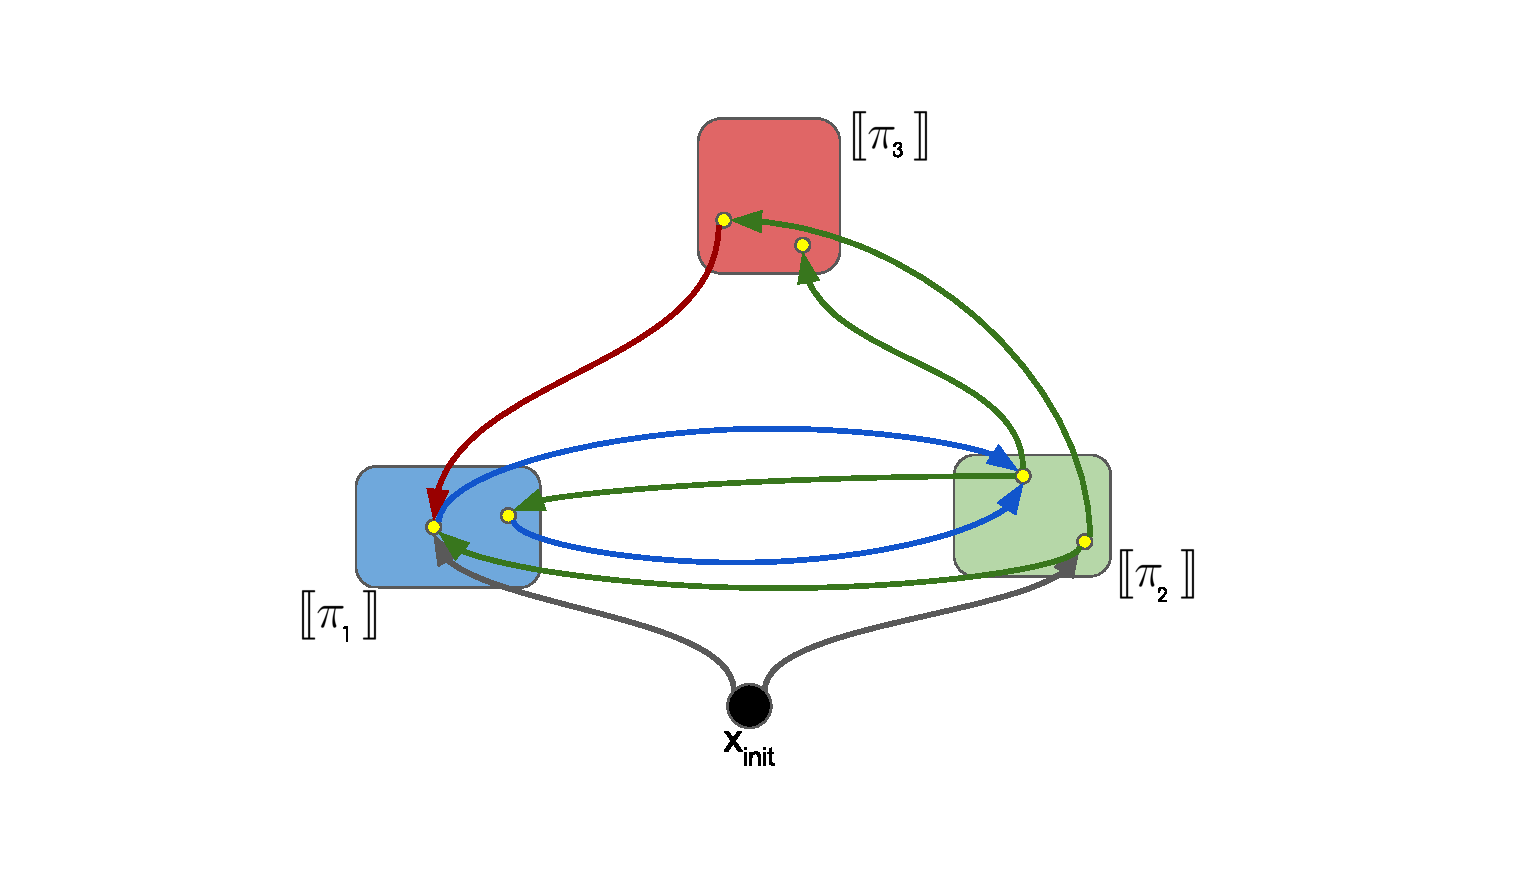
\includegraphics[scale=0.55]{./figures/quad_paths}
    \caption[Quadrotor planning with temporal logic specifications]{This diagram illustrates the set of solution trajectories found when attempting to reach from every sampled node of each proposition region (and initial state $x_{init}$) to all other proposition regions. We use $m=2$ samples in this example.}
\label{quad:fig:quad_paths}
\end{figure}

\begin{figure}[ht]
    \hspace*{-0.6cm}
    \centering
    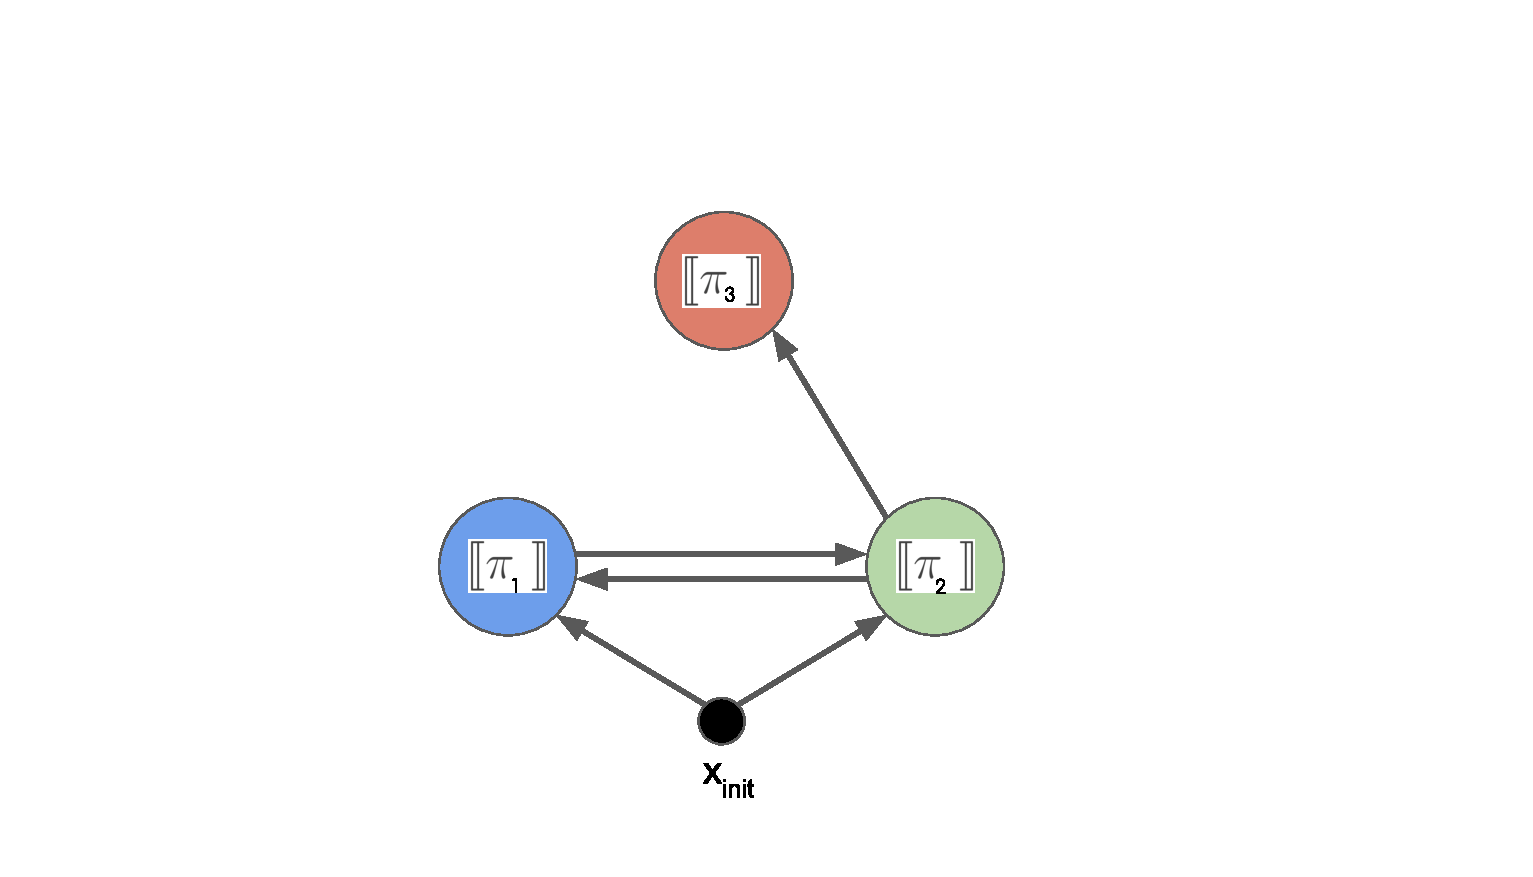
\includegraphics[scale=0.6]{./figures/quad_abstract_kripke}
    \caption[Abstracted Kripke structure for quadrotor paths]{Shown here is the abstracted Kripke structure based on the trajectories found in \autoref{quad:fig:quad_paths}. Note that an edge is only included when a solution is found from all samples of a given region to another particular region.}
\label{quad:fig:quad_abstract_kripke}
\end{figure}

It remains to determine whether or not the abstracted Kripke structure satisfies the given deterministic \mucalc{} specification. To this end, we once again use the local model checking algorithm from \autoref{chap:sstpaper} (\autoref{alg:modelchecking}). Once the appropriate set of transitions is determined, path smoothing can be applied. As we have not discussed how to generate smooth closed curves, which arise when any cycles are required in satisfying the specification, it suffices to plan each segment of the plan individually. At this point, the tracking controller from \autoref{quad:eqn:control_law} can be used to follow the proposed (possibly infinite) path. The quadrotor travels to the first proposition region, arriving at one of $m$ samples, and since each is guaranteed to have a known trajectory to the next destination, the quadrotor simply tracks the appropriate smooth path, and the process repeats as necessary. Note that this algorithm is reactive, and any newly appearing obstacles may necessitate finding new sets of waypoints to avoid collisions.
